\documentclass[../../main.tex]{subfiles}

\begin{document}

\subsection{Motivation}

%Each report must be created in a separate subfolder. Take the "example" folder as an example of a report (please do not change).
%
%Here it is required to describe the problematic of the problem. Basic premises and results. It is important to indicate a list of references on this topic~\cite{AuthorYear}. All refernces put to the main.bib file.
%
%After writing your report, include the report to main.tex similar to the sample report.

%All changes are made through GitHub\footnote{\url{https://github.com/Intelligent-Systems-Phystech/GeometricDeepLearning}}.

The work investigates the problem of predicting a complex structured target variable. The problem is supposed to be solved by higher-order partial least squares \cite{zhao2012higher}. This model predicts tensor $\underline{\mathbf{Y}}$ from tensor $\underline{\mathbf{X}}$ using projection into the latent space and solving regression problem on latent variables. The aim of computational experiment is to predict gyroscore data using accelerometer data. The experiment is held on a synthetic dataset. 

\subsection{Problem statement}

Given a dataset $\mathfrak{D} = (\underline{\mathbf{X}}, \underline{\mathbf{Y}})$, where tensors $\underline{\mathbf{X}} \in \mathbb{R}^{I_1\times \ldots\times I_N}$ and $\underline{\mathbf{Y}} \in \mathbb{R}^{J_1\times \ldots \times J_M}$, $I_1 = J_1$. We also require that $N \geq 3, ~M\geq 3$. Assume that $\underline{\mathbf{X}}$ is decomposed as a sum of rank-$(1, L_2, \ldots, L_N)$ Tucker-blocks, and $\underline{\mathbf{Y}}$ is decomposed as a sum of rank-$(1, K_2, \ldots, K_M)$ Tucker-blocks. This can be written in a following form:
\begin{equation}
\underline{\mathbf{X}} \approx \sum_{r=1}^R\underline{\mathbf{G}}_r\times_1\mathbf{t}_r\times_2\mathbf{P}^{(1)}_r\times_3\ldots \times_N\mathbf{P}_r^{(N - 1)},
\end{equation}

\begin{equation}
\underline{\mathbf{Y}} \approx \sum_{r=1}^R\underline{\mathbf{D}}_r\times_1\mathbf{t}_r\times_2\mathbf{Q}^{(1)}_r\times_3\ldots \times_M\mathbf{Q}_r^{(M - 1)},
\end{equation}
where $R$ is a number of latent vectors, $\mathbf{t}_r \in \mathbf{R}^{I_1}$ is a $r$-th latent vector, 
$\mathbf{P}_r^{(n)} \in \mathbb{R}^{I_{n+1}\times L_{n+1}}, ~\mathbf{P}_r^{(n)\top}\mathbf{P}_r^{(n)} = \mathbf{I}, ~\mathbf{Q}_r^{(m)} \in \mathbb{R}^{J_{m+1}\times K_{m + 1}}, ~\mathbf{Q}_r^{(m)\top}\mathbf{Q}_r^{(m)} = \mathbf{I}$, and $\underline{\mathbf{G}} \in \mathbb{R}^{1\times L_1\times \ldots \times L_N}, ~\underline{\mathbf{D}}\in \mathbb{R}^{1\times J_1\times K_1\times \ldots \times K_M}$ are core tensors.

For simplicity, let us define the following notation of Tucker decomposition:
\[
 \sum_{r=1}^R\underline{\mathbf{G}}_r\times_1\mathbf{t}_r\times_2\mathbf{P}^{(1)}_r\times_3\ldots \times_N\mathbf{P}_r^{(N - 1)} = [\underline{\mathbf{G}};\mathbf{t}, \mathbf{P}^{(1)}, \ldots, \mathbf{P}^{(N-1)}].
\]

Let $\underline{\mathbf{C}} \in \mathbb{R}^{I_2\times\ldots\times I_N\times J_2\times\ldots\times J_M}$, where:
\[
c_{i_2, \ldots, i_N, j_1, \ldots, j_M} = \sum_{i_1 = 1}^{I_1}x_{i_1, i_2, \ldots, i_N}y_{j_1, \ldots, j_M}.
\]
The problem is to find matrices $\underline{\mathbf{P}}_r^{(n)}, ~\underline{\mathbf{Q}}_r^{(m)}$ and latent vectors $\mathbf{t}_r$ from the following optimization problem:
\begin{equation}
\label{optim}
\max_{\mathbf{P}^{(n)}, \mathbf{Q}^{(m)}}\|[\underline{\mathbf{C}};\mathbf{P}^{(1)\top},\ldots,\mathbf{P}^{(N-1)\top}, \mathbf{Q}^{(1)\top}, \ldots, \mathbf{Q}^{(M-1)\top}]\|_F^2
\end{equation}
\begin{equation}
\mathrm{s.t.}, \quad \mathbf{P}^{(n)\top}\mathbf{P}^{(n)} = \mathbf{I}, ~\mathbf{Q}^{(m)\top}\mathbf{Q}^{(m)} = \mathbf{I}.
\end{equation}
Based on the found matrices $\underline{\mathbf{P}}^{(n)}, ~\underline{\mathbf{Q}}^{(m)}$ from \eqref{optim}, we find a latent vector $\mathbf{t}$ from the following optimization problem:
\begin{equation}
\mathbf{t} = \arg\min_{\mathbf{t}}\|\underline{\mathbf{X}} - [\underline{\mathbf{G}}; \mathbf{t}, \mathbf{P}^{(1)}, \ldots, \mathbf{P}^{(N - 1)}]\|_F^2.
\end{equation}
The following procedure should be carried $R$ times. The next step will be performed with a residual tensor:
\[
\underline{\mathbf{X}} - [\underline{\mathbf{G}}; \mathbf{t}, \mathbf{P}^{(1)}, \ldots, \mathbf{P}^{(N - 1)}].
\]

\subsection{Problem solution}
The optimization algorithm is described in \cite{zhao2012higher}. On each of $R$ steps it  computes orthogonal Tucker decomposition of $\underline{\mathbf{C}}_r$ and performs SVD decomposition in order to find $\mathbf{t}_r$. The algorithm may stop earlier when frobenius norm of both residuals is less than $\varepsilon$.

Prediction from a new observation $\underline{\mathbf{X}}^\text{test}$ can be written in matricized form:
\begin{equation}
\underline{\mathbf{Y}}_{(1)}^{\text{test}} = \mathbf{X}_{(1)}^\text{test}\mathbf{W}\mathbf{Q}^{*\top},
\end{equation}
where matrices $\mathbf{W}$ and $\mathbf{Q}$ have $R$ columns, which are the following:
\[
\mathbf{w}_r = (\mathbf{P}_r^{(N-1)}\otimes\ldots\otimes \mathbf{P}_r^{(1)})\underline{\mathbf{G}}_{r(1)}^+,
\]
\[
\mathbf{q}_r^* = \underline{\mathbf{D}}_{r(1)}(\mathbf{Q}_r^{(M-1)}\otimes\ldots\otimes\mathbf{Q}_r^{(1)})^\top.
\]

\subsection{Code analysis}

The implementation of HOPLS was taken from GitHub repository\footnote{https://github.com/arthurdehgan/HOPLS}. The computational experiment can be found on GitHub repository\footnote{https://github.com/Konstantin-Iakovlev/MathMethodsOfForecasting}.

\subsection{Experiment on synthetic dataset}

Consider an accelerometer tensor $\underline{\mathbf{X}}\in \mathbb{R}^{P\times T \times C}$, where $P = 10$ is a number of multivariate time series, $T = 40$ is a number of time steps, $C = 10$ is the number of channels. The task is to predict gyroscope data $\underline{\mathbf{Y}} \in \mathbb{R}^{P\times T \times C}$. Tensor $\underline{\mathbf{X}}$ was generated as:
\begin{equation}
x_{p, t, c} = \sin(\omega_{p, t, c} (t / T) + \varphi_{p,t, c}), \quad \omega_{p, t, c} \sim \mathcal{U}(20, 30), \quad \varphi_{p, t, c} \sim \mathcal{U}(0, \pi).
\end{equation}
Tensor $\underline{\mathbf{Y}}$ was generated as:
\begin{equation}
y_{p,t,c} = x_{p,t,c'}w_{c', c} + \varepsilon_{p,t,c},
\end{equation}
where $\mathbf{W} \in \mathbb{R}^{C\times C}, ~w_{c', c}\sim \mathcal{U}(0, 1), ~\varepsilon_{p,t,c}\sim \mathcal{N}(0, 0.01)$.


The task is to predict $\underline{\mathbf{Y}}$ by $\underline{\mathbf{X}}$, using method described above. Define a similarity between real $\underline{\mathbf{Y}}$ and $\underline{\mathbf{Y}}^\text{pred}$ as $Q^2$:
\begin{equation}
Q^2 = 1 - \frac{\|\underline{\mathbf{Y}}^\text{pred} - \underline{\mathbf{Y}}\|_F^2}{\|\underline{\mathbf{Y}}\|_F^2}.
\end{equation}

In order to measure quality of proposed method we performed cross validation. Here we split accelerometer data $\underline{\mathbf{X}}$ by the first dimension on 5 folds. In our model $L_2 = K_2 = 6, ~L_3 = K_3 =1$.

The goal of the computational experiment is to get dependence of validation quality on number of latent vectors $R$. We also compare proposed method with N-PLS. In fact, HOPLS can be simplified to N-PLS if we define all $L_n = 1$ and $K_m = 1$. 

\begin{table}
\caption{Dependence of $Q^2$ on $R$ on validation dataset}
\label{table}
\begin{tabular}{c|c|c|c|c|c|c|c|}
Method & $R= 1$ & $R= 4$ & $R = 10$ & $R = 13$ & $R = 16$ & $R = 19$\\ \hline
HOPLS  &0.41 $\pm$ 0.12 & 0.51 $\pm$ 0.19&  0.41 $\pm$ 0.12& 0.04 $\pm$ 0.47 & -0.22 $\pm$ 0.68&  -0.32 $\pm$ 0.68 \\
N-PLS & 0.42 $\pm$ 0.15 & 0.45 $\pm$ 0.11 & 0.35 $\pm$ 0.18 & 0.35 $\pm$ 0.19 & 0.33 $\pm$ 0.20 & 0.30 $\pm$ 0.20    
\end{tabular}
\end{table}

From Table \ref{table} it can be seen that HOPLS method gives better solution in terms of $Q^2$. In addition, variance of both methods is comparable.

From Figure \ref{fig:exp_1} it can be seen that the optimal $R^* = 4$. Moreover, the higher $R$ is, the more the variance of $Q^2$ is.
\begin{figure}[h!]
\centering
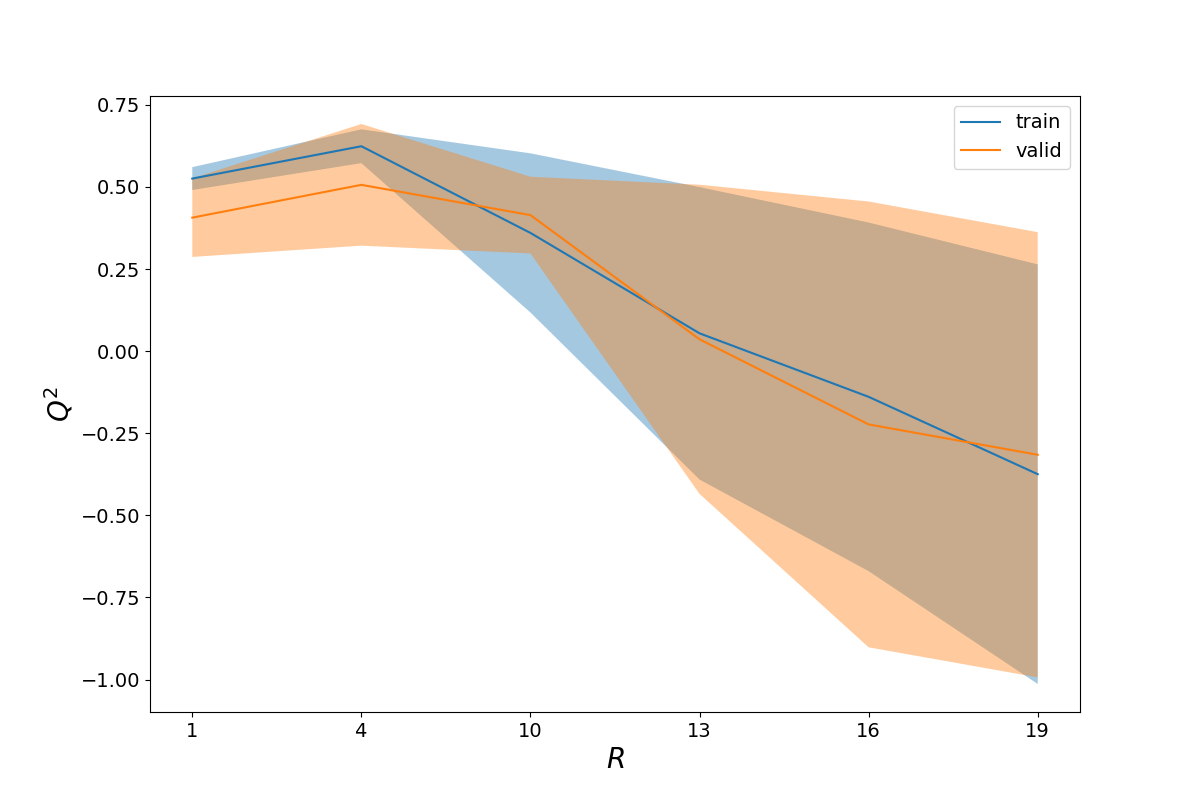
\includegraphics[width=1\textwidth]{figures/cross_val}
\caption{Dependence of $Q^2$ on number of latent vectors $R$.}
\label{fig:exp_1}
\end{figure}

%\begin{figure}[h!]
%\centering
%
\includegraphics[width=0.6\textwidth]{figures/fig1}
%\caption{Some description}
%\label{fig:example:1}
%\end{figure}
%
%This section requires some experiment analysis. The chapter assumes some graphs with their descriptions~\ref{fig:example:1}.

\end{document}